\documentclass[11pt,a4paper]{article}
\usepackage[margin=22mm]{geometry}
\usepackage{amsmath,amssymb,graphicx,xcolor,microtype}
\usepackage[hidelinks]{hyperref}
\usepackage{enumitem,fancyhdr}
\definecolor{accent}{HTML}{006C9E}
\setlength{\parindent}{0pt}
\setlength{\parskip}{6pt}
\setlist{itemsep=2pt,topsep=3pt,leftmargin=18pt}
\pagestyle{fancy}
\fancyhf{}
\fancyhead[L]{\small EPC2361 | Analytical loss model}
\fancyhead[R]{\small 75 V / 40 A RMS}
\fancyfoot[R]{\small\thepage}
\setlength{\headheight}{14pt}
\hypersetup{pdftitle={EPC2361 Half-Bridge Analytical Loss Modeling},pdfauthor={Analytical Loss Calculations - GaN}}
\begin{document}
{\LARGE\bfseries\color{accent} EPC2361 Half-Bridge\\[4pt]Analytical Loss Modeling}\par
{\large Updated operating point, loss equations and waveforms}\par
\textit{19 September 2026 | Implementation: epc2361\_loss.py and waveform\_plotter.py}

\section{Operating point and scope}
The model uses one EPC2361 in each of the two switch positions. The defaults are a
75 V DC bus, 40 A AC RMS current, 100 kHz switching frequency, sinusoidal PWM,
\textbf{modulation index $m=1$}, and unity power factor. The waveform factor $k_{\rm wf}=1$
scales the sinusoidal current amplitude; it does not model arbitrary harmonics.
The assumed half bridge has one hard turn-on/off pair per PWM period, with natural
commutation of the opposite device. This is a first-order estimate, not a DC-load model.

The retained circuit assumptions are 1 $\Omega$ external gate resistance in each
direction, 0.5 $\Omega$ source/sink driver resistance, 2 A driver current limits,
50 ns effective dead time, and 2 nH loop inductance. The default case temperature is
50 $^\circ$C and ambient temperature is 25 $^\circ$C.
\begin{align*}
 I_{\rm pk}&=\sqrt{2}\,I_{\rm rms}k_{\rm wf}=56.57\ {\rm A}, &
 I_{\rm avg,abs}&=\frac{2I_{\rm pk}}{\pi}=36.01\ {\rm A}.
\end{align*}
RMS current determines conduction loss; mean absolute current determines average
switching and dead-time loss. The plotted event defaults to peak current.

\section{Conduction loss and junction temperature}
The default \texttt{rds\_temperature\_mode=iterative} couples conduction loss to
junction temperature. The maximum 25 $^\circ$C resistance, 1.0 m$\Omega$, is selected
by default. At each iteration the normalized datasheet curve gives
\begin{align*}
 R_{\rm DS,on}(T_J)&=R_{\rm DS,on,25}\,k_T(T_J),\\
 d_{\rm dead}&=2t_{\rm dead,eff}f_{\rm sw}=0.01,\\
 P_{\rm cond}(T_J)&=I_{\rm rms}^{2}k_{\rm wf}^{2}R_{\rm DS,on}(T_J)(1-d_{\rm dead}),\\
 T_J^{(n+1)}&=T_{\rm ref}+\frac{R_\theta}{2}
 [P_{\rm cond}(T_J^{(n)})+P_{\rm overlap}+P_{\rm COSS}+P_{\rm dead}].
\end{align*}
The code starts at the selected case or ambient temperature and repeats until the
thermal residual is below $10^{-6}$ $^\circ$C, with a maximum of 200 iterations.
This numerical tolerance does not imply equivalent physical accuracy.

Piecewise-linear interpolation uses approximate readings of datasheet Figure 9 [1].
At 0, 25, 50, 75, 100, 125 and 150 $^\circ$C, the respective normalized factors are
0.84, 1.00, 1.16, 1.33, 1.49, 1.65 and 1.80.
The typical normalized curve scales the selected typical or maximum 25 $^\circ$C
resistance; it is not a guaranteed hot-resistance limit. No extrapolation is made
outside 0--150 $^\circ$C. Leaving that range or failing to converge produces an
explicit error instead of a reported steady-state solution.

The converged defaults are \textbf{$T_J=50.4922$ $^\circ$C},
\textbf{$R_{\rm DS,on}=1.16335$ m$\Omega$}, and $P_{\rm cond}=1.84274$ W
for both FETs combined. The small dead-time correction avoids double counting
normal conduction during reverse-conduction intervals. Optional external loop loss
is $P_{\rm loop}=I_{\rm rms}^{2}k_{\rm wf}^{2}R_{\rm loop}$.

Manual mode remains available and uses the entered multiplier (default 1.7) without
feedback. Iterative mode ignores that manual multiplier. The result reports updated
resistance, junction temperature, iteration count and residual. It estimates
steady-state temperature under the specified cooling conditions; it does not measure
actual junction temperature.

\newpage
\section{Device data and transition timing}
The supplied EPC2361 datasheet [1] gives typical/maximum on-resistance of
0.75/1.0 m$\Omega$, typical threshold voltage 1.1 V, internal gate resistance
0.4 $\Omega$, and zero reverse-recovery charge. At 50 V and 50 A, the gate-charge
values are $Q_G=28$ nC, $Q_{GS}=8.5$ nC, $Q_{G(th)}=6$ nC and $Q_{GD}=3.8$ nC.
Following AN030 [2],
\[
 Q_{GS2}=Q_{GS}-Q_{G(th)}=2.5\ {\rm nC}.
\]
The code uses an approximate plateau voltage $V_{PL}=2.1$ V from Figure 7.
At 75 V, integrating the small additional $C_{RSS}$ between 50 and 75 V gives
approximately $Q_{GD}=4.0$ nC and $Q_G=28.2$ nC. These are nominal curve-based
estimates. Plateau and current-transition charge remain fixed near the 50 A
characterization condition; exact current and temperature dependence is not solved.

With 5 V turn-on and 0 V turn-off drive, define
\begin{align*}
 R_{\rm on}&=R_{G,on}+R_{\rm driver,source}+R_{G,int}=1.9\ \Omega,\\
 R_{\rm off}&=R_{G,off}+R_{\rm driver,sink}+R_{G,int}=1.9\ \Omega,\\
 \bar V_G&=(V_{th}+V_{PL})/2.
\end{align*}
The gate-current estimates are separately limited by driver capability:
\begin{align*}
 I_{G,CR}&=\min\!\left(\frac{V_{DR}-\bar V_G}{R_{\rm on}},I_{\rm source}\right), &
 I_{G,VF}&=\min\!\left(\frac{V_{DR}-V_{PL}}{R_{\rm on}},I_{\rm source}\right),\\
 I_{G,VR}&=\min\!\left(\frac{V_{PL}}{R_{\rm off}},I_{\rm sink}\right), &
 I_{G,CF}&=\min\!\left(\frac{\bar V_G}{R_{\rm off}},I_{\rm sink}\right).
\end{align*}
The resulting current-rise, voltage-fall, voltage-rise and current-fall intervals are
\begin{align*}
 t_{CR}&=Q_{GS2}/I_{G,CR}=1.40\ {\rm ns}, &
 t_{VF}&=Q_{GD}/I_{G,VF}=2.62\ {\rm ns},\\
 t_{VR}&=Q_{GD}/I_{G,VR}=3.62\ {\rm ns}, &
 t_{CF}&=Q_{GS2}/I_{G,CF}=2.97\ {\rm ns}.
\end{align*}
Threshold and post-plateau segments use segment-average gate voltage and current
limits to complete the illustrative gate waveform. They are not exact nonlinear RC
transients, and the gate-charge segments must not exceed total $Q_G$.

\section{Switching overlap loss}
For an event at current $I_{\rm event}$, the triangular overlap approximation [2] is
\begin{align*}
 E_{\rm on}&=\tfrac12 V_{\rm bus}I_{\rm event}(t_{CR}+t_{VF}),\\
 E_{\rm off}&=\tfrac12 V_{\rm bus}I_{\rm event}(t_{VR}+t_{CF}).
\end{align*}
At 56.57 A these are 8.52 and 13.97 $\mu$J. The line-cycle average instead uses
$I_{\rm avg,abs}$:
\[
 P_{\rm overlap}=\tfrac12 V_{\rm bus}I_{\rm avg,abs}
 (t_{CR}+t_{VF}+t_{VR}+t_{CF})f_{\rm sw}=1.4323\ {\rm W}.
\]
Peak-current event energy is not applied to every PWM cycle.

\newpage
\section{Capacitor, gate-drive and dead-time losses}
For a symmetric half bridge, AN030 p6, Eqs17--18 [2], gives
\[
 P_{\rm COSS}=V_{\rm bus}Q_{\rm OSS}(V_{\rm bus})f_{\rm sw}=0.8550\ {\rm W}.
\]
Datasheet Figure 6 gives approximately $Q_{\rm OSS}=114$ nC and
$E_{\rm OSS}=3.2\ \mu$J at 75 V. The energy is reported for reference, not added
again. Neither small-signal $C_{\rm OSS}$ nor $Q_{\rm OSS}/V$ is an energy-equivalent
capacitance for a nonlinear device. When bus voltage changes, update the charge
and energy inputs to that voltage; mismatched charge-reference voltage is rejected.

The total gate-supply loss for the two FETs is
\[
 P_{\rm gate}=2Q_GV_{DR}f_{\rm sw}=0.0282\ {\rm W}.
\]
This energy is dissipated across the driver and gate resistances. Driver quiescent,
bootstrap and isolated-supply overhead are not included.

Using an approximate reverse drop $V_{SD}=2.2$ V from datasheet Figure 8,
\[
 P_{\rm dead}=2V_{SD}I_{\rm avg,abs}t_{\rm dead,eff}f_{\rm sw}=0.7923\ {\rm W}.
\]
The 1.6 V datasheet value applies at only 0.5 A. The selected 2.2 V is a representative
estimate at the modeled currents, not a fixed guaranteed drop. Effective dead time
may differ from commanded dead time in either direction [3]. Treating the entire
selected interval as reverse conduction is conservative: capacitor self-commutation
and duty-dependent distortion are not resolved. No reverse-recovery term is added.

\section{Total loss, efficiency and thermal result}
\begin{align*}
 P_{\rm loss}&=P_{\rm cond}+P_{\rm overlap}+P_{\rm COSS}
                 +P_{\rm gate}+P_{\rm dead}+P_{\rm loop}\\
             &=4.9505\ {\rm W},\\
 V_{\rm out,rms}&=\frac{mV_{\rm bus}}{2\sqrt{2}}=26.5165\ {\rm V},\\
 P_{\rm out}&=V_{\rm out,rms}I_{\rm rms}\,\mathrm{PF}=1060.66\ {\rm W},\\
 \eta&=100\frac{P_{\rm out}}{P_{\rm out}+P_{\rm loss}}=99.5354\%.
\end{align*}
These efficiency figures include only the modeled losses, not all converter/system
losses. Output voltage uses the retained sinusoidal half-bridge convention.

The thermal calculation excludes external loop and gate-supply losses:
\begin{align*}
 P_{\rm semi}&=P_{\rm cond}+P_{\rm overlap}+P_{\rm COSS}+P_{\rm dead},\\
 P_{\rm device}&=P_{\rm semi}/2=2.46114\ {\rm W},\\
 T_J&=T_{\rm case}+P_{\rm device}R_{\theta JC}=50.4922\ {^\circ\rm C}.
\end{align*}
Equal sharing applies to symmetric sinusoidal averaging. The default
$R_{\theta JC}=0.2\ {^\circ\rm C/W}$ assumes the case is maintained at 50 $^\circ$C.
Ambient mode instead uses $T_J=T_{\rm amb}+P_{\rm device}R_{\theta JA}$ with
44 $^\circ$C/W for the JEDEC board (25 $^\circ$C/W for the datasheet EVB).
The small internal-gate-resistance share is omitted from junction heating.
Conduction loss is recomputed with the converged resistance. The other loss terms
remain fixed during iteration; temperature dependence of gate charge, reverse drop
and switching energy is not modeled.

\newpage
\section{Waveforms, slew rates and voltage stress}
\begin{center}
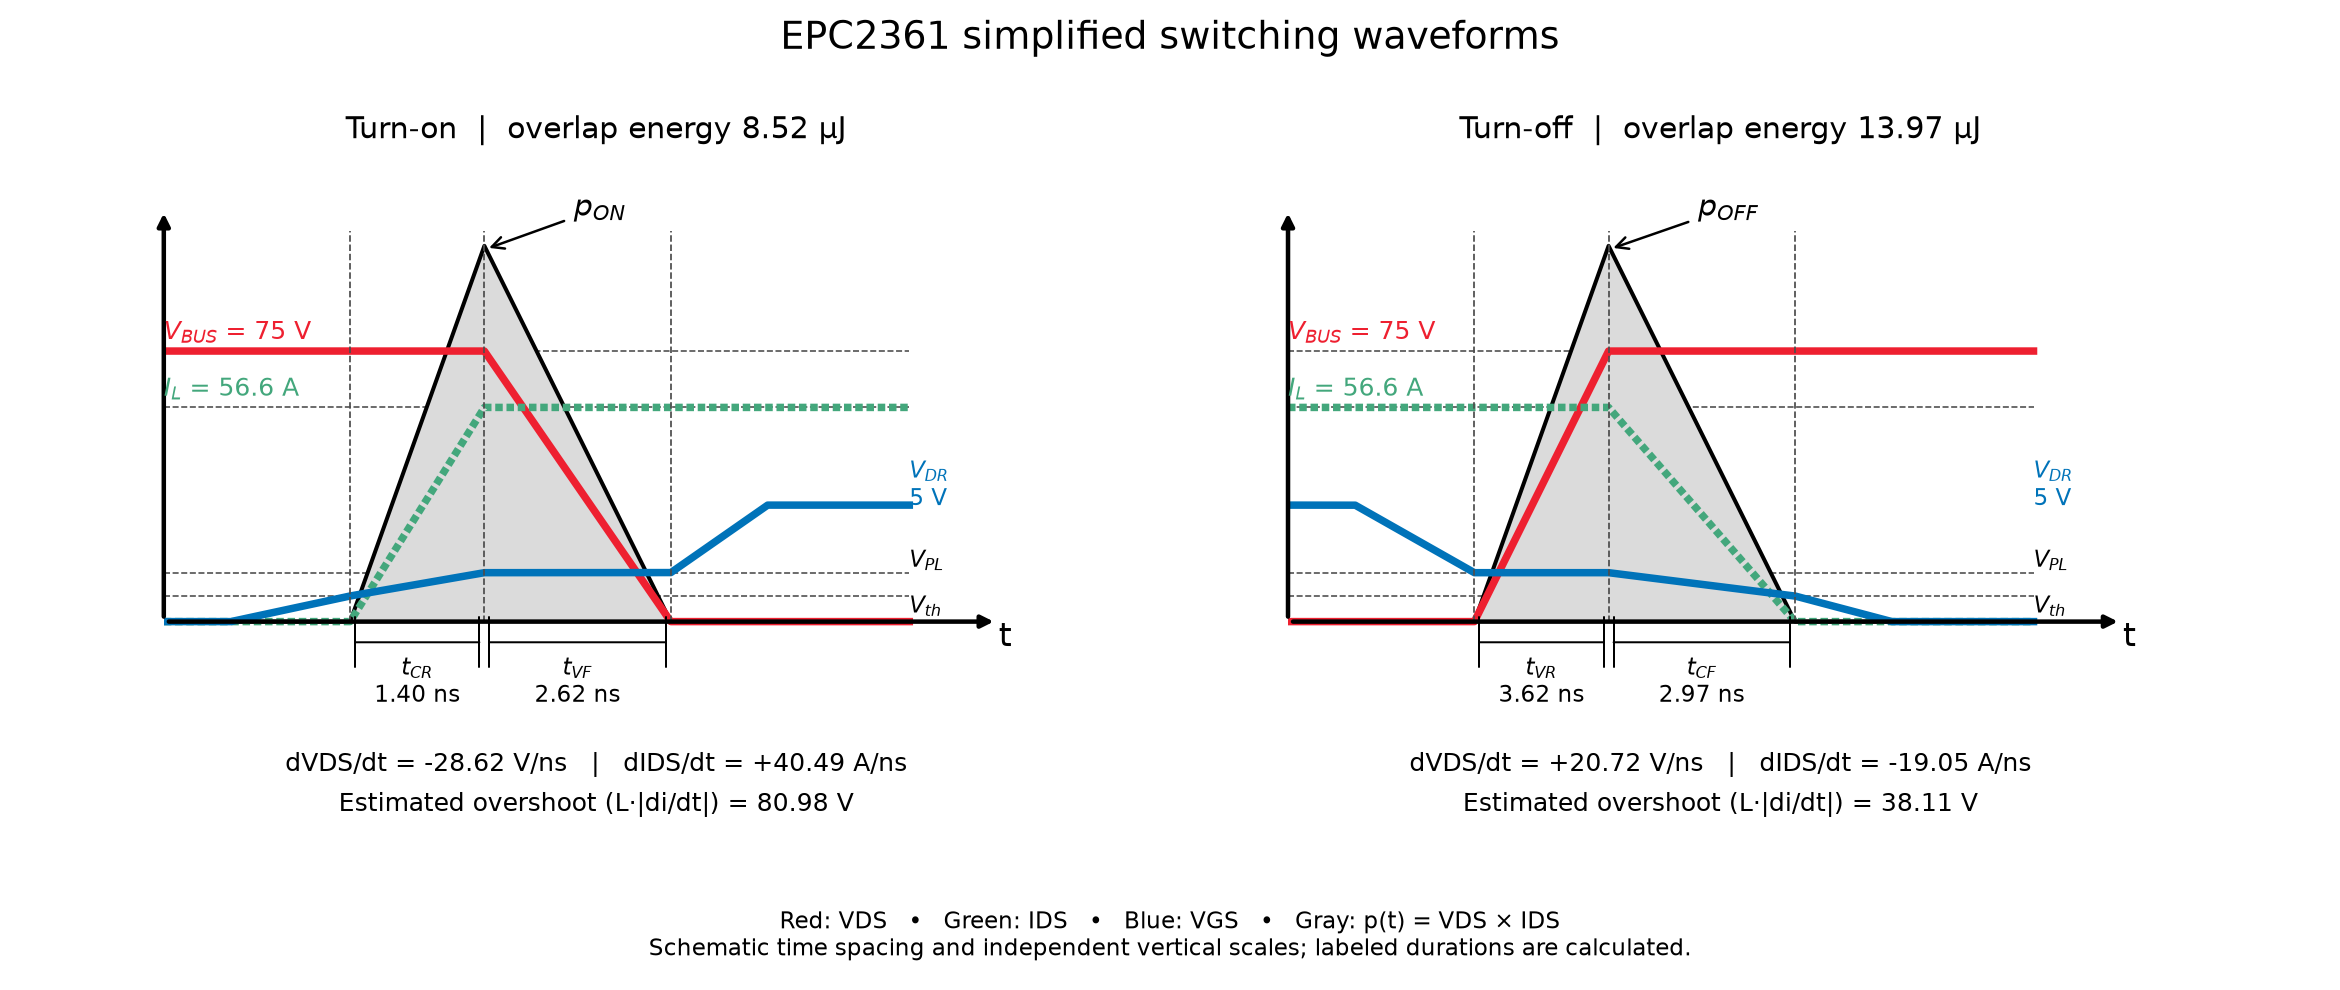
\includegraphics[width=\textwidth]{output/switching_waveforms.png}
\end{center}
\textit{Figure 1.} Simplified turn-on and turn-off waveforms following AN030
Figures 2--3. Time spacing and vertical scales are schematic; the labeled intervals
and slew rates are calculated. Gray shading represents channel overlap power.
The physical-time waveform arrays integrate to the reported event energies.

The signed slopes refer to $V_{DS}$ and $I_{DS}$ in their respective transition
intervals. The overshoot indicators use their current-slope magnitudes:
\begin{align*}
 \Delta V_{\rm on}&=L_{\rm loop}\frac{I_{\rm event}}{t_{CR}}=80.98\ {\rm V},\\
 \Delta V_{\rm off}&=L_{\rm loop}\frac{I_{\rm event}}{t_{CF}}=38.11\ {\rm V},\\
 V_{\rm stress}&=V_{\rm bus}+\max(\Delta V_{\rm on},\Delta V_{\rm off})
                =155.98\ {\rm V}.
\end{align*}
This crude estimate exceeds the device's 100 V continuous rating. The retained
2 nH input is exposed rather than adjusted to suppress the result. The calculation
does not solve nonlinear commutation, common-source inductance, damping or gate
feedback, so it is not a prediction of a measured voltage peak. Validate timing and
stress with a parasitic-aware model and double-pulse measurements [4].

Disabling hard switching suppresses both overlap and capacitor dissipation as an
ideal fully soft-switched limit; it does not establish ZVS. Optional LC ringing is
illustrative and does not change the analytical loss accounting. Thermal transients,
PCB/heatsink spreading, dynamic on-resistance and driver overhead remain outside
the model. Ten numerical checks cover loss accounting, waveform integration, input handling,
thermal balance, an independent closed-form solution and failure conditions.

\section*{References}
\small
[1] EPC, \emph{EPC2361 Datasheet}, revised 20 July 2026: pp1--2 for ratings and
charge data; p3, Figures5--9 for capacitance, charge, reverse conduction and temperature.

[2] EPC, AN030, \emph{Hard Switching Losses Calculation}: pp2--5 for gate-charge
transitions and overlap; p6 for capacitor and gate-drive loss.

[3] EPC, \emph{Dead-Time Optimization for Maximum Efficiency}, p1.

[4] EPC, \emph{eGaN FET Drivers and Layout Considerations}; \emph{Impact of
Parasitics on Performance}; AN023, \emph{Accurately Measuring High Speed GaN
Transistors}; \emph{Thermal Performance of eGaN FETs}.
\end{document}
